A network system can be represented as a simple graph $G(V,E)$ where $V$ is the set of nodes that includes $H$ end hosts and $R$ routers. $E$ is the set of links. 
Due to scalability or privacy constraints, deploying monitoring capabilities at every point of the targeted large-scale network is not possible. Therefore, the problem can be concisely modeled as a bipartite mapping graph between the path level flows and its network components as shown in Fig.~\ref{fig:bipartite}. 

We further observe that one component failure (e.g., $L_j$) will cause multiple paths erroneous while one flow error (e.g., $F_i$) may be caused by multiple component failures. And because the component gray failure probability is normally low ($10^{-3} - 10^{-6}$), it would require a large number of file transfers to catch a few corrupted files. Our ultimate goal is to localize the possible root causes in node or link errors by inference from the observed flow level abnormalities only at the end hosts, which can be translated to learning the mappings in such a graph.

\begin{wrapfigure}{ht}{0.25\textwidth}
  \begin{center}
    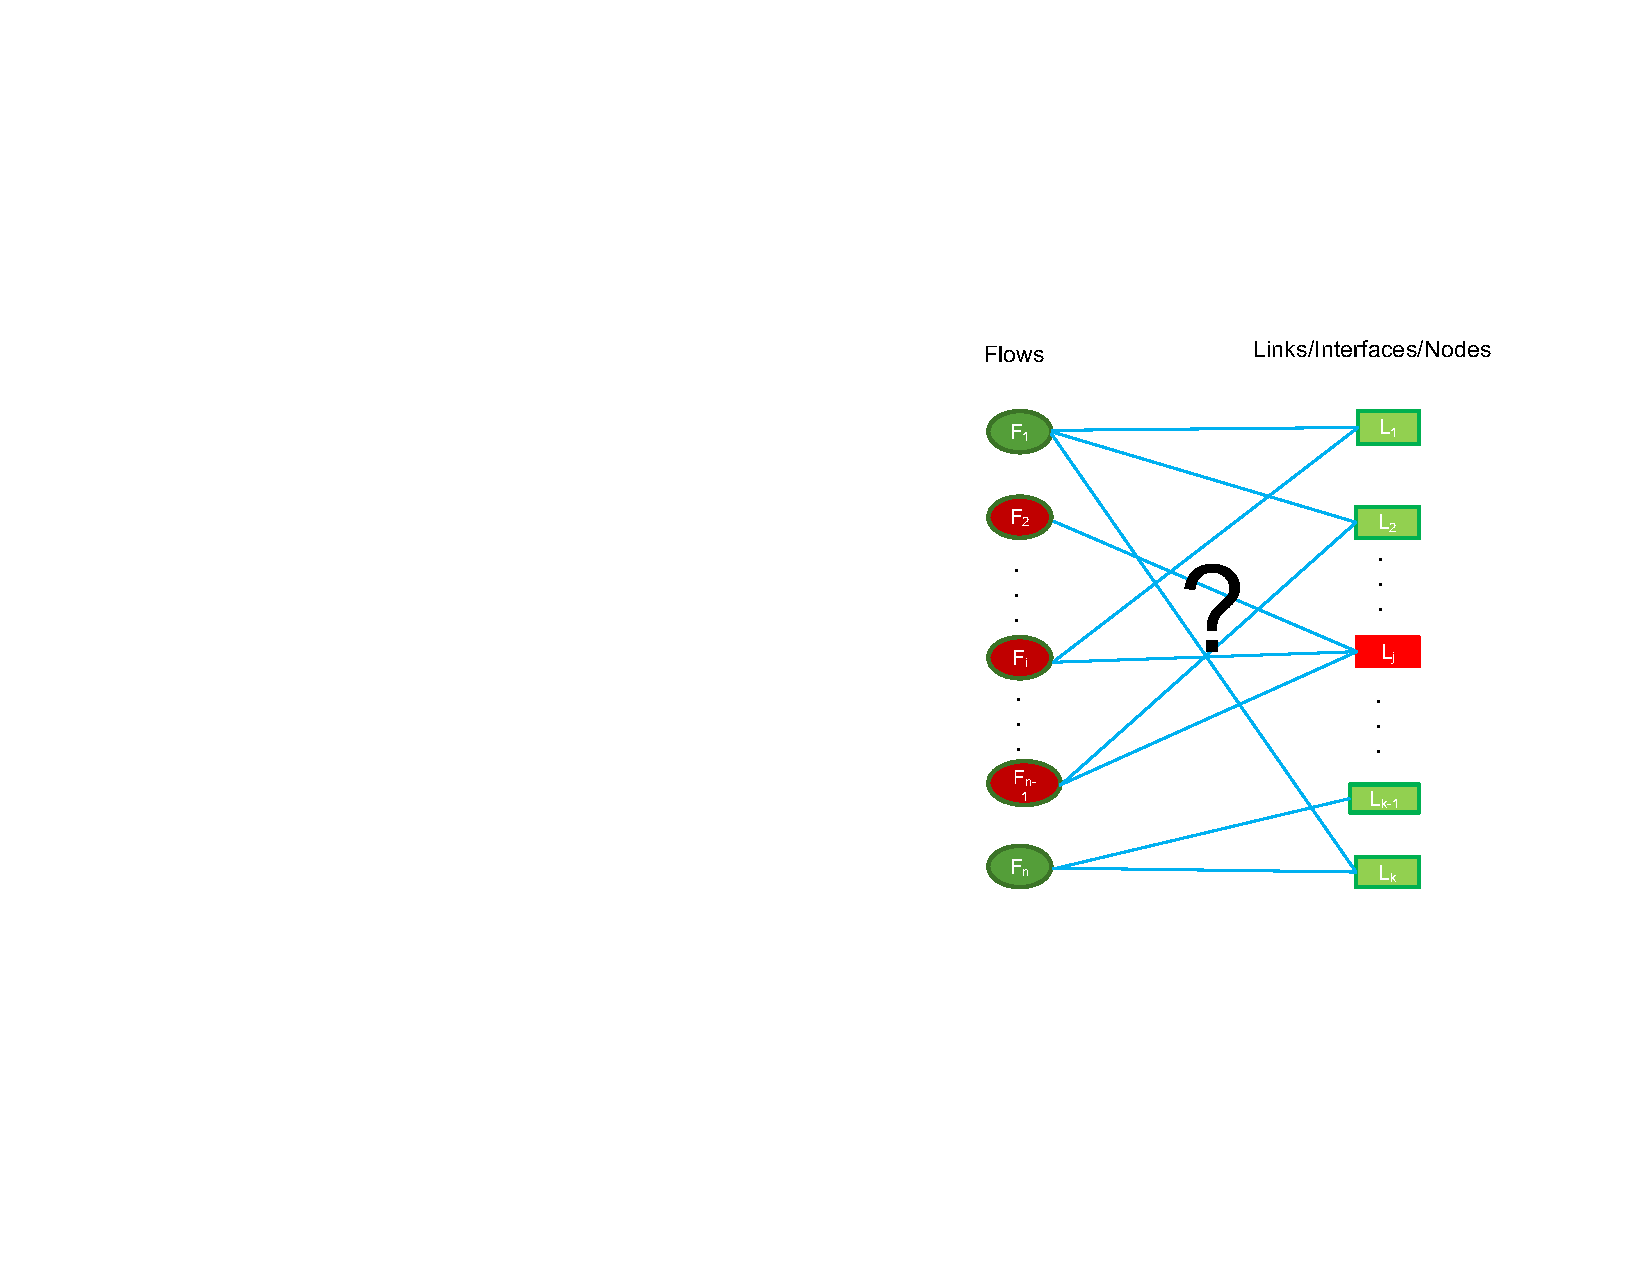
\includegraphics[width=0.25\textwidth]{./figure/RCABipartite}
  \end{center}
  \vspace{-5pt}
\caption{RCA Bipartite Graph}
\vspace{-5pt}
\label{fig:bipartite}
\end{wrapfigure}

In general, the fundamental network RCA problem is to use the path-level measurement to deduce the faulty components that can be concisely modeled by the formula~\ref{eq:prob}.
A path $P_i$ that a file transfer (flow) $i$ traverses consists of origin node $H_i^o$, a set of links where each $e_i^{\tilde{j}}\in E$ has two interfaces $e_i^t$ and $e_i^r$ on the route, and destination node $H_i^d$. 
As our main concern is if a file is corrupted rather than packet losses, the file characteristics, $F_i$, \eg, the source and destination nodes, file size, transfer time, retransmission, etc. all become part of the data features. 
Some of the features are continuous variables and some are categorical variables.
As the components ($\tilde{j}$) of $P\ i$ that file transfer $i$ traverses is unknown except for its two end hosts $H_i^o$ and $H_i^d$, the model actually needs to implicitly learn the file routes in order to infer the root causes.   
As a result, we can not use the traditional stochastic learning approach.

\begin{flalign}\label{eq:prob}
\begin{aligned}
&Probability(File\ i\ corrupted) =\\
&f(F_i, \prod_{\tilde{j} \in P_i}Probability(device\ \tilde{j}\ is\ faulty) )
\end{aligned}
\end{flalign}

The majority of recent studies assume flow information between any pair of nodes in the network is available because they focus on data center networks that they have full ownership and their modern routers allow originating and receiving probing data. This is very important because, as shown in~\cite{netbouncer:nsdi18}, there exists a minimal set of source-destination pairs to guarantee successful pinpointing of link errors in the network. They further assume the routes for all flows are known, i.e., the mapping represented in Fig.~\ref{fig:bipartite}. However, both assumptions do not hold for our targeted Internet environment due to obvious administrative constraints, complex topology, and the lack of monitoring coverage. In the Internet-scale network, traffic routing and forwarding paths are hard to obtain because of frequent topology and policy changes, the widely adaptation of multi-path routing, and disabled {\it Ping} and {\it Traceroute} in many places~\cite{arzani2018democratically}. Furthermore, deployment of a monitoring infrastructure to conduct system-wide active and passive monitoring is administratively and costly prohibitive.     

What makes problem problem unique is that the flow routes are unknown, \ie, thee mapping relationship in~\ref{fig:bipartite} is unknown.
However, the file level measurement and characteristics give us extra data features that could enhance the model accuracy, which is the case that we'll show in the evaluation. 

In summary we made more restrictive but more realistic assumptions in this study in that (1) only the data file transfer information including integrity error states can be obtained at the end hosts from the application layer; (2) only the physical nodes (or abstract representation of domains) and their interfaces are known to us, but the network topology and traffic routing are unknown. 









